%% V1.0
%% by Gabriel Garcia, gabrcg@gmail.com
%% This is a template for Udacity projects using IEEEtran.cls

%% Be Udacious!

\documentclass[10pt,journal,compsoc]{IEEEtran}

\usepackage[pdftex]{graphicx}    
\usepackage{cite}
\usepackage{url}
\hyphenation{op-tical net-works semi-conduc-tor}


\begin{document}

\title{American Sign Language interaction with Robot}

\author{Jeremy Hale}

\markboth{Inference project, Robotic Nanodegree, Udacity}%
{}
\IEEEtitleabstractindextext{%

\begin{abstract}
There are roughly half a million users of American Sign Language (ASL)\cite{wiki:asl}. With the growing presence of companion robots in the world, it is necessary for the Deaf to be able to communicate with Robots using ASL.

We present a method for recognizing the hand gestures used in ASL to represent the latin alphabet using neural networks.
\end{abstract}

% Note that keywords are not normally used for peerreview papers.
\begin{IEEEkeywords}
Robot, IEEEtran, Udacity, \LaTeX, deep learning.
\end{IEEEkeywords}}


\maketitle
\IEEEdisplaynontitleabstractindextext
\IEEEpeerreviewmaketitle
\section{Introduction}
\label{sec:introduction}

\IEEEPARstart{W}{hile} detailed research into the history of communication between deaf persons and robots was not conducted, the need for this communication to exist is readily apparent. The data science website, Kaggle, has a dataset for mnist using ASL\cite{kaggle:mnist_asl}, however, a new dataset was created to fulfill the requirements of the project. Furthemore, the Kaggle dataset is in tabular form as opposed to image form and not ready to be used with convolutional neural networks.

The dataset includes the entire latin alphabet except for letters "j" and "z" which require motion. A neural network that reconigzes motion gestures is beyond the scope of the project.

\begin{figure}[thpb]
      \centering
      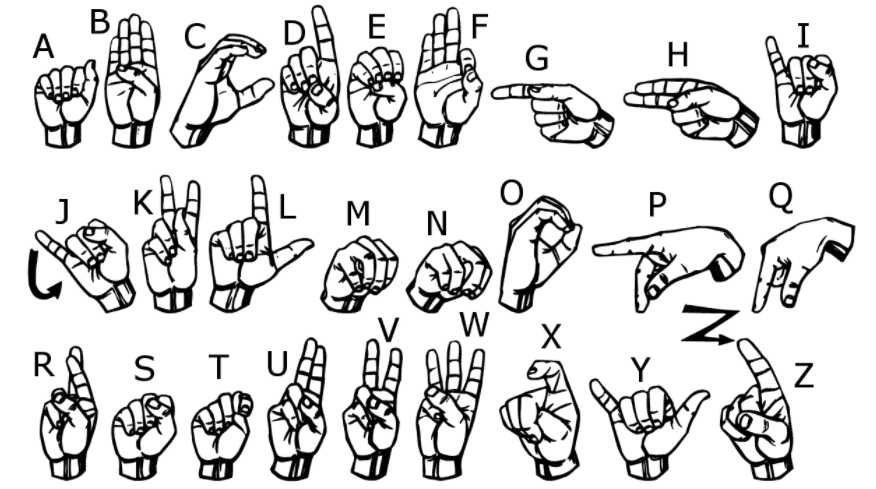
\includegraphics[width=\linewidth]{american_sign_language}
      \caption{American Sign Language.\cite{kaggle:mnist_asl}}
      \label{fig:asl}
\end{figure}

\section{Background / Formulation}
The dataset was classified using a LeNet\cite{Lecun98gradient-basedlearning} network which is available as a standard network in the nVidia DIGITS application. The network is a simple 2 block network with each block consisting of a convolutional neural network (CNN) followed by max pool layer. The CNNs have kernel size 5 and stride 1, while the max pool layers have kernel size 2 and stride 2. The CNN blocks connect to a fully-connected layer with 500 units followed by a fully-connected with the number of units equal to the number of classes.

The number of epochs was set to 30 while the learning rate was the default 0.01.

In general, the network with the fewest parameters that yields sufficient accuracy should be chosen. In this case, the LeNet is the simplest model available and was able to perform satisfactorily.

\section{Data Acquisition}
The nVidia Jetson TX2 was used for acquiring a dataset of 11,000 images. The udacity-modification of Peter Morgan's code\cite{PeterMoran} was programmed on to the TX2 and then used to capture images of the author's hand in various ASL poses. Approximately 400 images of each letter gesture were capture for the dataset.

The images were captured using the builtin camera on the TX2 against a white wall. The author attempted to keep their body and face outside of the field of view and to rotate their hand as well as move their hand around the field of view to generate a variety of camera angles.

\begin{figure}[thpb]
      \centering
      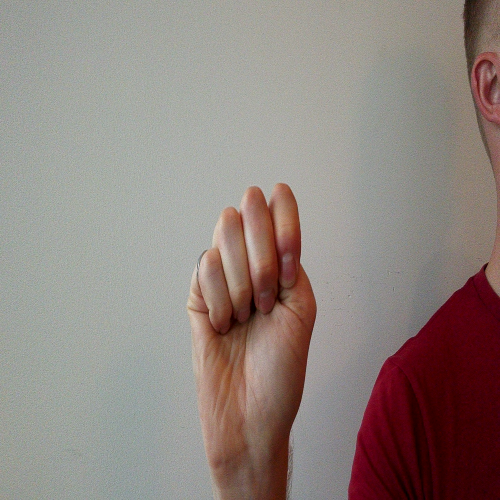
\includegraphics[width=\linewidth]{test_4127}
      \caption{Letter "M".}
      \label{fig:letter_m}
\end{figure}

The images were then resized to 28 x 28 using Python code from \cite{Budy} to work with the expected input size for LeNet. Using nVidia DIGITS, the images were imported into a dataset of 8272 training images and 2755 validation images. They were imported as grayscale images.

\section{Results}

The LeNet network achieved greater than 99 percent accuracy on the validation data after only 5 epochs.

\begin{figure}[thpb]
      \centering
      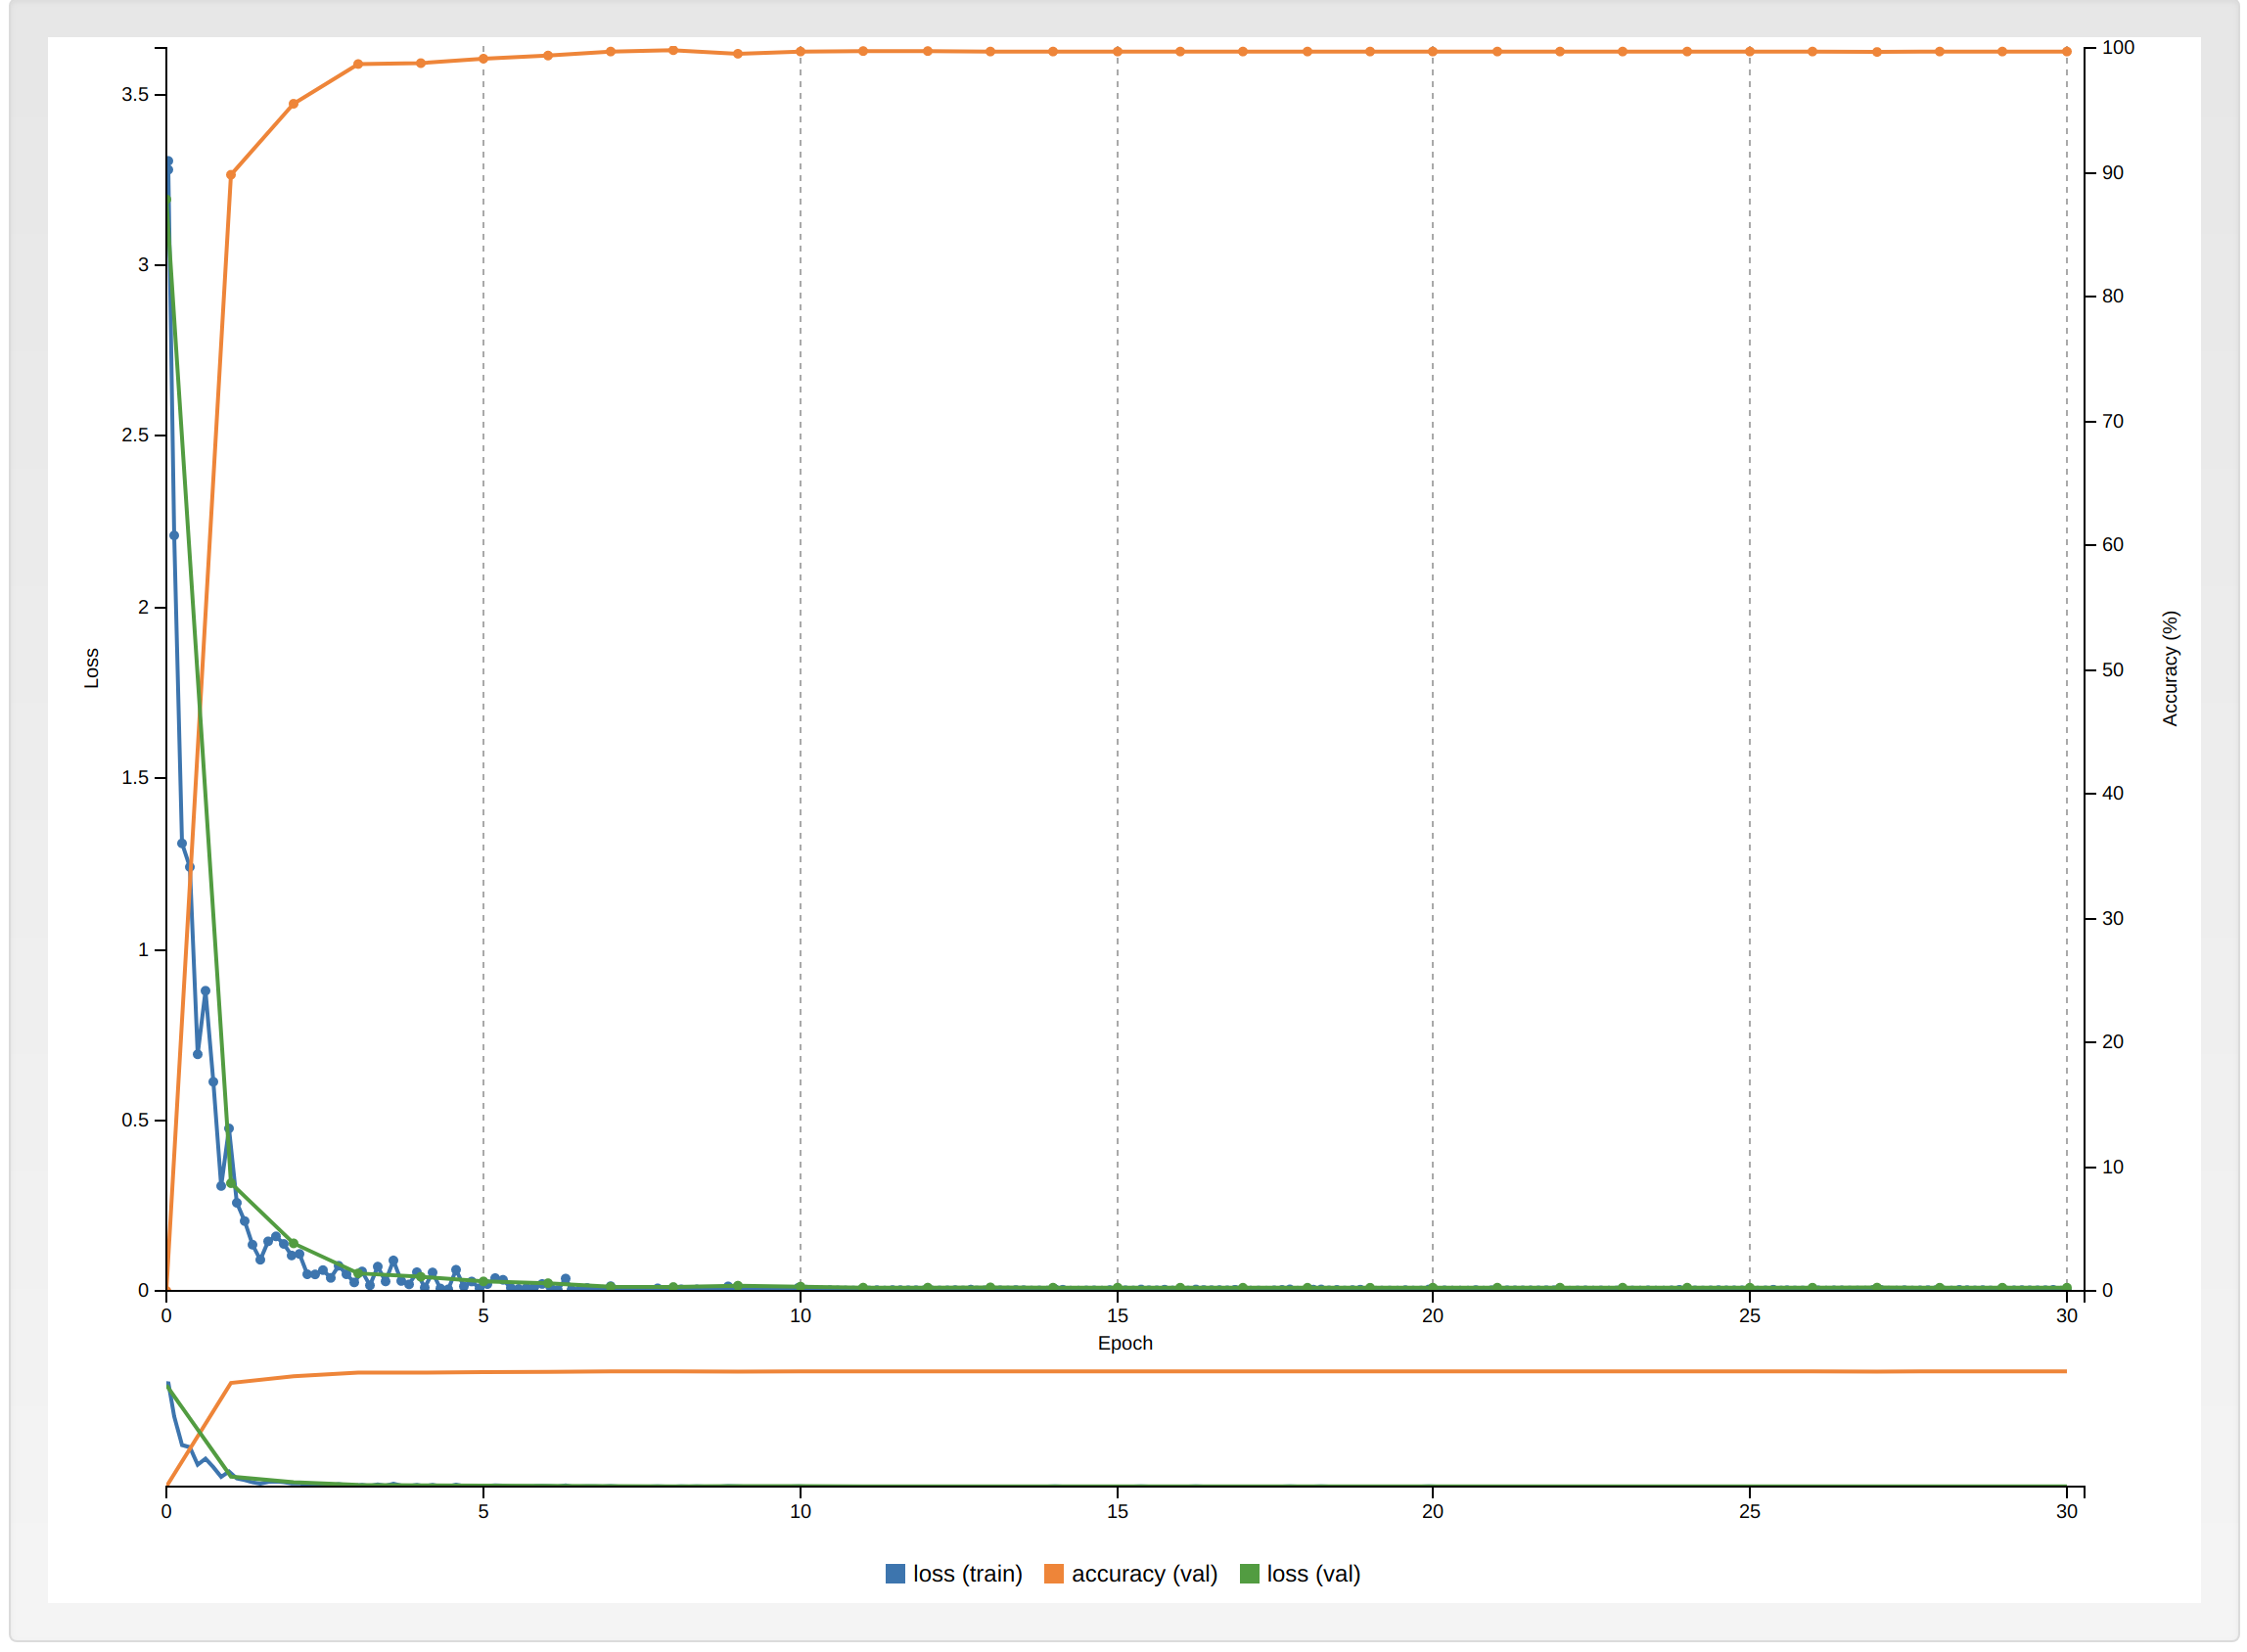
\includegraphics[width=\linewidth]{lenet_results}
      \caption{Results.}
      \label{fig:results}
\end{figure}


\section{Discussion}
The excellent results are likely due to the limitations of the dataset. The dataset most likely has similarities between images in the same class that are not related to the hand gesture being made. For example, the author's red shirt is visible in most the the label "M" images but not other labels. It's possible the network was able to "cheat" by learning to recognize the presence of the shirt instead of the position of the hand.

\section{Conclusion / Future work}
The work presented here shows that it is indeed feasible to have a robot recognize the ASL alphabet and that a simple CNN-based network can be employed accurately.

For a real-world application, the network would need to be improved to not only recognize the letters "J" and "Z" which include motion, but also to include an entire vocabularly of ASL words, many of which include motion.

\bibliography{bib}
\bibliographystyle{ieeetr}

\end{document}